% Provenance (never printed): see sources/outline_sources.md (Year 2: metamorphic reactions,
% Clapeyron slopes, the Al2SiO5 diagram, the facies grid, protoliths). Definitions and facies
% table from the IUGS subcommission proposal (via the Granada translation); thermodynamic data
% from Robie and Hemingway (1995); experimental diagram from Holdaway and Mukhopadhyay (1993);
% curves from figdata/bachelor-2/facies.py; exercise and problem values in the Book 4 scratch
% calculator calc/ch10.py.
\chapter{Metamorfe reacties en facies}\label{ch:b2:metamorphic-facies}

Een basalt die met zijn plaat wegzinkt, blijft geen basalt. Zijn plagioklaas en pyroxeen
reageren, in vaste toestand, tot andere mineralen, en de nieuwe associatie hangt af van de
druk en de temperatuur die hij bereikte: een blauw gesteente van glaucofaan en lawsoniet, of een
groen-rood gesteente van omfaciet en granaat. Metamorfe gesteenten houden deze mineralen wanneer
ze naar het oppervlak terugkeren, en een petroloog die de reacties kent, kan er de
omstandigheden uit aflezen. Dit hoofdstuk schrijft die reacties met de thermodynamica van de
scheikundecursus, berekent uit gemeten gegevens het beroemdste metamorfe fasediagram,
dat van de drie \ce{Al2SiO5}-mineralen, vergelijkt het met het experiment, en ordent de
associaties van metamorfe gesteenten in facies.
% ledger: scmr:facies-assemblages

\begin{recall}
\textbf{Uit Boek~2}: \omterm{def:b2:metamorphic-facies:metamorphism}{metamorfose}, metamorfe graad, indexmineralen
en isograden, contactmetamorfose en haar \omterm{def:b2:magma-emplacement:aureole}{contacthof}, foliatie en schistositeit,
lithostatische druk; kyaniet, andalusiet en sillimaniet als polymorfen, en hun
fasediagram. \textbf{Uit de natuurkunde- en scheikundeboeken van het eerste jaar universiteit}: de
gibbsenergie $G = H - TS$, waarvan het minimum de stabiele toestand bij gegeven $T$ en $P$ aangeeft;
enthalpie, entropie en warmtecapaciteit; $\mathrm dG = V\,\mathrm dP - S\,\mathrm dT$; de
betrekking van Clausius--Clapeyron voor het verdampen van een zuivere stof en het
tripelpunt van water. \textbf{Uit Boek~3}: subductiezones, botsingsgordels en
de geotherm.
\end{recall}

\section{Metamorfose}\label{sec:b2:metamorphic-facies:metamorphism}

Boek~2 behandelde \omterm{def:b2:metamorphic-facies:metamorphism}{metamorfose} als de omvorming van een gesteente door warmte en
druk. Een internationale aanbeveling geeft de definitie die hier wordt gebruikt.

\begin{definition}[Metamorfose; protoliet]\label{def:b2:metamorphic-facies:metamorphism}
\emph{Metamorfose}\index{metamorfose} is een proces dat de mineralen of de
microstructuur van een gesteente verandert, of beide, in wezen in vaste toestand, terwijl het gesteente zich aanpast
aan fysische omstandigheden die verschillen van die waaronder het ontstond en van die
welke normaal aan het aardoppervlak en in de diagenesezone heersen. Ze kan samengaan met
\omterm{def:b2:mantle-melting:melting}{partieel smelten} en kan de chemische samenstelling van het gesteente veranderen. Het gesteente vóór de
metamorfose is zijn \emph{protoliet}\index{protoliet}.
\end{definition}
% ledger: scmr:metamorphism

De ondergrens sluit diagenese uit, de veranderingen van een sediment terwijl het wordt begraven en
verhardt, en de bovengrens is smelten, bestudeerd in \cref{ch:b2:crustal-melting}. De
factoren zijn temperatuur, druk, de fluïda die door het gesteente circuleren (water en
koolstofdioxide vooral) en vervorming. \omterm{def:b2:metamorphic-facies:metamorphism}{Metamorfose} wordt ingedeeld naar haar omvang en
haar omgeving.
% ledger: scmr:metamorphism, scmr:types

\emph{Regionale} \omterm{def:b2:metamorphic-facies:metamorphism}{metamorfose} treft grote volumes gesteente en gaat samen met grootschalige
tektonische processen: ze is \emph{orogeen} in gebergtegordels, waar korst bij een
botsing verdikt; \emph{begravingsmetamorfose} treft gesteenten die diep zijn begraven onder dikke
sedimentaire of vulkanische pakketten, zonder vervorming of magmatisme, zodat haar gesteenten
meestal geen schistositeit hebben; \emph{oceaanbodemmetamorfose} verandert de korst bij
spreidingsruggen, waar heet zeewater er onder steile thermische
gradiënten doorheen circuleert, en haar herkristallisatie is meestal onvolledig. \emph{Lokale} \omterm{def:b2:metamorphic-facies:metamorphism}{metamorfose}
heeft een lokale oorzaak: \emph{contactmetamorfose} verhit het nevengesteente van een intrusie;
\emph{hydrothermale} \omterm{def:b2:metamorphic-facies:metamorphism}{metamorfose} wordt aangedreven door hete, waterrijke fluïda;
\emph{dislocatiemetamorfose}, in breuk- en schuifzones, verkleint de korrelgrootte en
maakt mylonieten en cataclasieten; \emph{inslagmetamorfose}, onder een meteorietinslag,
kan gesteente doen smelten en verdampen. \omterm{def:b2:metamorphic-facies:metamorphism}{Metamorfose} heet prograde zolang de temperatuur stijgt en
retrograde zolang die daalt.
% ledger: scmr:types

\section{Metamorfe reacties}\label{sec:b2:metamorphic-facies:reactions}

\begin{definition}[Metamorfe reactie; devolatilisatiereactie]\label{def:b2:metamorphic-facies:reaction}
Een \emph{metamorfe reactie}\index{metamorfe reactie} zet een verzameling mineralen
van een gesteente, de reactanten, om in een andere verzameling, de producten, in vaste toestand, eventueel
met deelname van een fluïde fase. Een \emph{devolatilisatiereactie}\index{devolatilisatiereactie}
is een reactie die een vluchtige stof vrijmaakt, water bij een dehydratatiereactie of
koolstofdioxide bij een decarbonatatiereactie.
\end{definition}

In dit hoofdstuk komen drie typen voor. Polymorfe omzettingen, zoals kyaniet naar
sillimaniet of calciet naar aragoniet, behouden de formule en veranderen de structuur.
Andere reacties tussen vaste stoffen herverdelen componenten over mineralen, zoals
albiet dat jadeïet plus kwarts geeft:
\[
\ce{NaAlSi3O8 -> NaAlSi2O6 + SiO2}.
\]
\omterm{def:b2:metamorphic-facies:reaction}{Devolatilisatiereacties} maken een fluïdum vrij, zoals muscoviet en kwarts die bij hoge
temperatuur uiteenvallen:
\[
\ce{KAl3Si3O10(OH)2 + SiO2 -> KAlSi3O8 + Al2SiO5 + H2O}.
\]
% ledger: day73:ms-qz

Voor een reactie tussen mineralen met vaste samenstelling is de verandering van de gibbsenergie
$\Delta_r G(T, P) = \sum G_{\text{producten}} - \sum G_{\text{reactanten}}$; de producten
zijn stabiel waar $\Delta_r G < 0$, de reactanten waar $\Delta_r G > 0$, en de twee
bestaan naast elkaar waar $\Delta_r G = 0$.

\begin{definition}[Univariante reactie]\label{def:b2:metamorphic-facies:univariant}
Een reactie tussen fasen met vaste samenstelling is \emph{univariant}\index{univariante reactie}
wanneer haar evenwichtsvoorwaarde $\Delta_r G(T, P) = 0$ één variabele
vrij laat: het evenwicht is een lijn in het druk--temperatuurvlak, die
het veld van de reactanten scheidt van dat van de producten.
\end{definition}

\begin{definition}[Clapeyronhelling]\label{def:b2:metamorphic-facies:clapeyron}
De \emph{Clapeyronhelling}\index{Clapeyronhelling} van een reactie is de helling
$\mathrm dP/\mathrm dT$ van haar evenwichtslijn in het druk--temperatuurvlak.
\end{definition}

\begin{proposition}[Clapeyronhelling van een reactie]\label{prop:b2:metamorphic-facies:clapeyron}
Langs de evenwichtslijn van een reactie met entropieverandering $\Delta_r S$ en
volumeverandering $\Delta_r V$ geldt
\[
\frac{\mathrm dP}{\mathrm dT} = \frac{\Delta_r S}{\Delta_r V}.
\]
\end{proposition}

\begin{proof}
Voor elke fase geldt $\mathrm dG = V\,\mathrm dP - S\,\mathrm dT$, dus voor de reactie
$\mathrm d(\Delta_r G) = \Delta_r V\,\mathrm dP - \Delta_r S\,\mathrm dT$. Langs de lijn
blijft $\Delta_r G = 0$ nul: $\Delta_r V\,\mathrm dP = \Delta_r S\,\mathrm dT$.
\end{proof}

Dit is de betrekking van Clausius--Clapeyron uit de natuurkunde, geschreven voor vaste stoffen. Met
$\Delta_r S$ in \unit{J.mol^{-1}.K^{-1}} en $\Delta_r V$ in \unit{J.bar^{-1}} (één
\unit{J.bar^{-1}} is \qty{10}{cm^3}) komt de helling uit in bar per kelvin. Twee
gevolgen bepalen elk metamorf fasediagram. Tussen vaste stoffen zijn de entropie- en
volumeveranderingen klein, zodat een reactielijn steil of vlak kan zijn, positief of
negatief: de hogetemperatuurkant bevat de producten met de hogere entropie, en de
hogedrukkant die met het kleinere volume. Bij een \omterm{def:b2:metamorphic-facies:reaction}{devolatilisatiereactie} brengt het fluïdum
een grote entropie mee, dus de producten liggen aan de hogetemperatuurkant; en het volume
van het fluïdum, groot bij lage druk en krimpend naarmate de druk stijgt, maakt de helling
vlak bij lage druk en steiler bij hoge druk. De reactielijn buigt.
Experimenten met muscoviet en kwarts plaatsen haar op 603, 637 en \qty{662}{\celsius} bij 1,
2 en \qty{3}{kbar} waterdruk: tussen 1 en \qty{2}{kbar} klimt de lijn
\qty{29}{bar} per kelvin, tussen 2 en 3 \qty{40}{bar} (\cref{exo:b2:metamorphic-facies:9}).
% ledger: day73:ms-qz

\section{De aluminiumsilicaten}\label{sec:b2:metamorphic-facies:al2sio5}

\begin{definition}[Aluminiumsilicaatpolymorfen]\label{def:b2:metamorphic-facies:al2sio5}
De \emph{aluminiumsilicaatpolymorfen}\index{aluminiumsilicaatpolymorfen} zijn de drie
mineralen met formule \ce{Al2SiO5}: kyaniet (triclien), andalusiet en sillimaniet (beide
orthorombisch).
\end{definition}
% ledger: rh95:al2sio5

Ze komen veel voor in gemetamorfoseerde kleistenen, waarvan ze het aluminium dragen, en omdat ze
dezelfde formule hebben, hangt het alleen van druk en temperatuur af welke ervan groeit. De tabel
hieronder geeft hun gemeten eigenschappen.

\begin{center}
\small
\begin{tabular}{@{}lrrrr@{}}
\hline
 & $\Delta_f H^\circ$ (\unit{kJ.mol^{-1}}) & $S^\circ$ (\unit{J.mol^{-1}.K^{-1}}) & $V^\circ$ (\unit{J.bar^{-1}}) & dichtheid (\unit{g.cm^{-3}})\\
\hline
kyaniet & $-2593.8$ & 82.80 & 4.415 & 3.670\\
andalusiet & $-2589.9$ & 91.39 & 5.152 & 3.145\\
sillimaniet & $-2586.1$ & 95.40 & 4.986 & 3.250\\
\hline
\end{tabular}
\par\smallskip{\small Kyaniet, andalusiet en sillimaniet bij \qty{298.15}{K} en
\qty{1}{bar} (Robie en Hemingway, 1995); de enthalpieën zijn onzeker tot op
\qty{2.0}{kJ.mol^{-1}}, de entropieën tot op 0.5. Dichtheid uit de molaire massa,
\qty{162.046}{g.mol^{-1}}, en het volume.}
\end{center}
% ledger: rh95:al2sio5

Kyaniet is het dichtst en heeft de minste entropie: het is de hogedruk-,
lagetemperatuurpolymorf. Andalusiet, het minst dicht, beheerst lage druk; sillimaniet,
met de hoogste entropie, beheerst hoge temperatuur. Hun evenwichtslijnen zijn te berekenen.

\begin{method}[Een reactielijn berekenen]\label{met:b2:metamorphic-facies:line}
(1) Vorm uit de tabellen $\Delta_r H$, $\Delta_r S$ en $\Delta_r V$ bij \qty{298.15}{K}
en \qty{1}{bar}. (2) Verwaarloos de verandering van $\Delta_r H$ en $\Delta_r S$ met de
temperatuur (warmtecapaciteiten van producten en reactanten bijna gelijk) en van $\Delta_r V$
met druk en temperatuur (vaste stoffen worden nauwelijks samengedrukt of zetten nauwelijks uit):
\[
\Delta_r G(T, P) \approx \Delta_r H - T\,\Delta_r S + \Delta_r V\,(P - 1).
\]
(3) Stel dit gelijk aan nul: $P = 1 + (T\,\Delta_r S - \Delta_r H)/\Delta_r V$, een rechte lijn met
helling $\Delta_r S/\Delta_r V$. (4) Vervang, waar precisie telt, $\Delta_r H$ en
$\Delta_r S$ door hun waarden bij de temperatuur $T$, uit tabellen van $H_T - H_{298}$ en $S_T$,
en los opnieuw op. (5) Houd van elke lijn alleen het deel over waar haar twee fasen stabieler zijn
dan elke derde.
\end{method}

Voor kyaniet naar andalusiet is $\Delta_r H = \qty{3.9}{kJ}$, $\Delta_r S =
\qty{8.59}{J.K^{-1}}$ en $\Delta_r V = \qty{0.737}{J.bar^{-1}}$: bij \qty{25}{\celsius}
en \qty{1}{bar} is $\Delta_r G = 3900 - 298.15\times8.59 = \qty{+1.34}{kJ}$, dus kyaniet,
niet andalusiet, is de stabiele polymorf aan het aardoppervlak; kyaniet naar sillimaniet heeft
daar $\Delta_r G = \qty{+3.94}{kJ}$. De hellingen zijn $8.59/0.737 = \qty{11.7}{bar/K}$ voor
kyaniet naar andalusiet, $12.60/0.571 = \qty{22.1}{bar/K}$ voor kyaniet naar sillimaniet en
$4.01/(-0.166) = \qty{-24.2}{bar/K}$ voor andalusiet naar sillimaniet, de enige reactie van
de drie waarvan het hogetemperatuurproduct het dichtst is.
% ledger: rh95:al2sio5

\begin{definition}[Invariant punt]\label{def:b2:metamorphic-facies:invariant}
Een \emph{invariant punt}\index{invariant punt} is een punt van het
druk--temperatuurvlak waar drie of meer fasen van een systeem in
evenwicht naast elkaar bestaan en alle \omterm{def:b2:metamorphic-facies:univariant}{univariante lijnen} ertussen samenkomen; er is daar geen variabele vrij.
\end{definition}

\begin{proposition}[Het tripelpunt]\label{prop:b2:metamorphic-facies:triple}
De drie lijnen kyaniet $=$ andalusiet, kyaniet $=$ sillimaniet en andalusiet $=$
sillimaniet komen samen in één punt. Rond dat punt is elke lijn maar aan één kant stabiel; haar
metastabiele verlenging ligt in het veld van de derde polymorf.
\end{proposition}

\begin{proof}
Voor elke $(T, P)$ geldt $\Delta G_{\text{ky}\to\text{sil}} = \Delta G_{\text{ky}\to\text{and}} +
\Delta G_{\text{and}\to\text{sil}}$, omdat de gibbsenergieën van andalusiet tegen elkaar wegvallen. Waar
de eerste twee lijnen elkaar snijden, verdwijnen twee van deze termen, dus de derde ook: de derde
lijn gaat door het snijpunt. Voorbij het snijpunt geldt, op de lijn kyaniet $=$ andalusiet
bijvoorbeeld, $G_{\text{ky}} = G_{\text{and}}$, maar het punt ligt aan de sillimanietkant van de
twee andere lijnen, dus $G_{\text{sil}}$ is kleiner dan beide: kyaniet noch andalusiet
is daar stabiel, en de lijn is metastabiel.
\end{proof}

Met de constante eigenschappen van de methode ligt het tripelpunt op
\qty{514}{\celsius} en \qty{3.88}{kbar} (het weekendprobleem); met de
temperatuurafhankelijkheid uit de tabellen op \qty{536}{\celsius} en \qty{4.20}{kbar}. Het experimentele
diagram, opgebouwd uit omgekeerde experimenten, plaatst het op $504 \pm \qty{20}{\celsius}$ en
$3.75 \pm \qty{0.25}{kbar}$ (de figuur hieronder).
% ledger: rh95:al2sio5-ht, hm93:triple, hm93:table11

\begin{omfigure}
\centering
\begin{tikzpicture}
\begin{axis}[omrecord, width=0.84\linewidth, height=7.4cm,
  xmin=200, xmax=900, ymin=0, ymax=10, xlabel={$T$ (\unit{\celsius})}, ylabel={$P$ (\unit{kbar})},
  legend style={font=\scriptsize, at={(0.02,0.98)}, anchor=north west},
  tick label style={font=\scriptsize}, label style={font=\small}]
\addplot[very thick, blue!70!black] table[x=T_C, y=P_kbar] {figdata/out/bachelor-2-facies-stable-kyand.dat};
\addlegendentry{berekend (tabellen)}
\addplot[thick, gray, densely dashed, mark=o, mark size=1.2pt] table[x=T_C, y=P_kbar] {figdata/out/bachelor-2-facies-hm93-kyand.dat};
\addlegendentry{experimenteel}
\addplot[thick, orange!85!black, mark=square*, mark size=1.3pt] table[x=T_C, y=P_kbar] {figdata/out/bachelor-2-facies-day73.dat};
\addlegendentry{muscoviet + kwarts}
\addplot[very thick, blue!70!black, forget plot] table[x=T_C, y=P_kbar] {figdata/out/bachelor-2-facies-stable-kysil.dat};
\addplot[very thick, blue!70!black, forget plot] table[x=T_C, y=P_kbar] {figdata/out/bachelor-2-facies-stable-andsil.dat};
\addplot[thin, blue!70!black, dashed, forget plot] table[x=T_C, y=P_kbar] {figdata/out/bachelor-2-facies-meta-kyand.dat};
\addplot[thin, blue!70!black, dashed, forget plot] table[x=T_C, y=P_kbar] {figdata/out/bachelor-2-facies-meta-kysil.dat};
\addplot[thin, blue!70!black, dashed, forget plot] table[x=T_C, y=P_kbar] {figdata/out/bachelor-2-facies-meta-andsil.dat};
\addplot[thick, gray, densely dashed, mark=o, mark size=1.2pt, forget plot] table[x=T_C, y=P_kbar] {figdata/out/bachelor-2-facies-hm93-kysil.dat};
\addplot[thick, gray, densely dashed, mark=o, mark size=1.2pt, forget plot] table[x=T_C, y=P_kbar] {figdata/out/bachelor-2-facies-hm93-andsil.dat};
\addplot[only marks, mark=*, mark size=2pt, blue!70!black, forget plot] table[x=T_C, y=P_kbar] {figdata/out/bachelor-2-facies-triple-B.dat};
\addplot[only marks, mark=*, mark size=2pt, gray, forget plot] table[x=T_C, y=P_kbar] {figdata/out/bachelor-2-facies-hm93-triple.dat};
\node[font=\small\bfseries] at (axis cs:330,6.2) {kyaniet};
\node[font=\small\bfseries] at (axis cs:460,0.6) {andalusiet};
\node[font=\small\bfseries] at (axis cs:790,3.6) {sillimaniet};
\end{axis}
\end{tikzpicture}
\par\smallskip{\small Het \ce{Al2SiO5}-diagram berekend uit de thermodynamische tabellen van
Robie en Hemingway (1995) met temperatuurafhankelijke enthalpie en entropie (blauw; gestreept:
metastabiele verlengingen), en het experimentele diagram van Holdaway en Mukhopadhyay (1993)
(grijs, hun getabelleerde punten). Oranje: het uiteenvallen van muscoviet + kwarts, gemeten door
Day (1973), dat buigt.}
\end{omfigure}
% ledger: rh95:al2sio5, rh95:al2sio5-ht, hm93:table11, hm93:triple, day73:ms-qz

De berekende lijn kyaniet--andalusiet valt tussen 400 en \qty{600}{\celsius} binnen \qty{0.1}{kbar} van de experimentele,
maar de lijn andalusiet--sillimaniet ligt
bij \qty{600}{\celsius} \qty{0.65}{kbar} te hoog. Die lijn is de kwetsbaarste van de
drie: met $\Delta_r V = \qty{-0.166}{J.bar^{-1}}$ verschuift een fout van \qty{0.1}{kJ} in
$\Delta_r H$, een twintigste van de onzekerheid van elke enthalpie in de tabel, haar met
\qty{600}{bar}. De enthalpieën van de tabellen zijn zelf aan de
experimenten aangepast, binnen hun onzekerheden; de experimenten, niet de calorimetrie alleen, leggen het
diagram vast.
% ledger: rh95:al2sio5, hm93:adjusted, hm93:table11

De figuur hieronder toont waarom een lijn een grens is. Bij \qty{6}{kbar} gaan de gibbsenergieën van
andalusiet en sillimaniet, gemeten ten opzichte van die van kyaniet, door nul waar elk
stabieler zou worden dan kyaniet; de verschillen zijn nooit groter dan enkele kilojoules per mol,
wat verklaart waarom een kleine fout in een enthalpie een lijn zo ver verschuift.

\begin{omfigure}
\centering
\begin{tikzpicture}
\begin{axis}[omrecord, width=0.7\linewidth, height=5.4cm,
  xmin=300, xmax=900, ymin=-4, ymax=4.5, xlabel={$T$ (\unit{\celsius})},
  ylabel={$G - G_{\text{kyaniet}}$ (\unit{kJ.mol^{-1}})},
  legend style={font=\scriptsize, at={(0.02,0.02)}, anchor=south west},
  tick label style={font=\scriptsize}, label style={font=\small}]
\addplot[very thick, red!75!black] table[x=T_C, y=dG_and] {figdata/out/bachelor-2-facies-dg6.dat};
\addlegendentry{andalusiet}
\addplot[very thick, green!45!black] table[x=T_C, y=dG_sil] {figdata/out/bachelor-2-facies-dg6.dat};
\addlegendentry{sillimaniet}
\addplot[thin, black] coordinates {(300,0) (900,0)};
\end{axis}
\end{tikzpicture}
\par\smallskip{\small Gibbsenergieën van andalusiet en sillimaniet ten opzichte van kyaniet bij
\qty{6}{kbar}, uit dezelfde tabellen. Kyaniet is stabiel zolang beide krommen positief zijn;
sillimaniet neemt het over bij \qty{624}{\celsius}. Andalusiet gaat pas door nul bij
\qty{692}{\celsius}, waar sillimaniet al lager ligt: boven de druk van het
tripelpunt is andalusiet nooit het stabielst.}
\end{omfigure}
% ledger: rh95:al2sio5, rh95:al2sio5-ht

\begin{inthelab}[Een reactie omkeren]
Een reactielijn wordt in het laboratorium gelokaliseerd met experimenten bij vaste druk en
temperatuur die uitgaan van een mengsel van reactanten en producten. In een
zuiger--cilinderapparaat wordt het mengsel een tot enkele dagen vastgehouden; de richting van de reactie wordt daarna
afgelezen met röntgendiffractie, door de verhouding van de pieken van product en reactant
te vergelijken met die van het beginmengsel, en bevestigd door aangroei op het stabiele mineraal. Andere
studies wegen een enkel kristal andalusiet dat in een poeder van kyaniet of
sillimaniet heeft gereageerd, met een microbalans die tot op ongeveer \qty{4}{\micro g} nauwkeurig is. Een evenwicht is
\emph{omgekeerd} wanneer groei van elke kant is waargenomen aan weerszijden van de lijn;
de lijn ligt dan in het interval ertussen, getekend met de fouten van het apparaat,
typisch \qty{10}{\celsius} en \qty{0.5}{kbar}. Experimentatoren beoordelen een fasediagram eerst
aan zulke omkeringen, en pas daarna aan de gesteenten.
\end{inthelab}
% ledger: hm93:methods

\section{Associaties en facies}\label{sec:b2:metamorphic-facies:facies}

\begin{definition}[Minerale associatie]\label{def:b2:metamorphic-facies:assemblage}
Een \emph{minerale associatie}\index{minerale associatie} is de verzameling mineralen die
samen in evenwicht zijn gegroeid in een metamorf gesteente.
\end{definition}

Een associatie hangt af van de omstandigheden van de \omterm{def:b2:metamorphic-facies:metamorphism}{metamorfose} en van de samenstelling van het
gesteente. Eskola, die in 1915 het faciesbegrip invoerde, zag dat gesteenten van dezelfde
samenstelling onder dezelfde omstandigheden dezelfde associatie dragen, en dat de
associaties van verschillende gesteenten samen veranderen wanneer de omstandigheden veranderen; de
internationale aanbeveling behoudt zijn begrip.
% ledger: scmr:facies

\begin{definition}[Metamorfe facies; faciesrooster]\label{def:b2:metamorphic-facies:facies}
Een \emph{metamorfe facies}\index{metamorfe facies} is een verzameling metamorfe \omterm{def:b2:metamorphic-facies:assemblage}{minerale
associaties}, herhaaldelijk samen in tijd en ruimte, die een regelmatig verband vertonen
tussen minerale samenstelling en totale chemische samenstelling, zodat verschillende facies
overeenkomen met verschillende metamorfe omstandigheden, vooral temperatuur en druk. De
facies worden benoemd en gedefinieerd aan de hand van de associaties van gesteenten met basaltische samenstelling. Een
\emph{faciesrooster}\index{faciesrooster} is de rangschikking van de facies in het
druk--temperatuurvlak.
\end{definition}
% ledger: scmr:facies

De tabel hieronder geeft tien facies met hun diagnostische mineralen in metabasalten.

\begin{center}
\small
\begin{tabular}{@{}p{0.27\linewidth}p{0.66\linewidth}@{}}
\hline
facies & diagnostische mineralen van een metabasalt\\
\hline
zeoliet & zeolieten zoals laumontiet en heulandiet\\
prehniet--pumpellyiet & prehniet + pumpellyiet, prehniet + actinoliet, pumpellyiet + actinoliet\\
groenschist & actinoliet + albiet + chloriet + epidoot\\
epidoot-amfiboliet & hoornblende + albiet + epidoot $\pm$ chloriet\\
amfiboliet & hoornblende + plagioklaas (meer dan \qty{17}{\percent} anorthiet)\\
granuliet & clinopyroxeen + orthopyroxeen + plagioklaas; olivijn niet stabiel met plagioklaas of granaat\\
blauwschist & glaucofaan + epidoot $\pm$ granaat, of glaucofaan + lawsoniet\\
eclogiet & omfaciet + granaat; plagioklaas niet stabiel\\
pyroxeenhoornrots & clinopyroxeen + orthopyroxeen + plagioklaas; olivijn stabiel met plagioklaas\\
sanidiniet & hetzelfde, met mineralen van zeer hoge temperatuur zoals pigeoniet\\
\hline
\end{tabular}
\par\smallskip{\small De facies en hun diagnostische associaties in gesteenten met basaltische
samenstelling, naar de internationale aanbeveling (de acht facies van Eskola, met de
zeolietfacies en de prehniet--pumpellyietfacies later toegevoegd).}
\end{center}
% ledger: scmr:facies-assemblages, scmr:facies

De aanbeveling benadrukt wat de facies niet doen: ze leggen regelmatigheden tussen
associaties vast, en proberen niet de druk en temperatuur van elke facies vast te leggen. Hun volgorde in
het druk--temperatuurvlak volgt uit de reacties ertussen, en de
figuur hieronder tekent haar schematisch. De temperatuur stijgt van de zeolietfacies via
de groenschist- en amfibolietfacies naar de granulietfacies; bij lage druk en hoge
temperatuur liggen de hoornrotsfacies van contacthoven; bij hoge druk en lage
temperatuur de blauwschistfacies; bij hoge druk en hogere temperatuur de
eclogietfacies. Reacties uit dit hoofdstuk leggen stukken van de grenzen vast: plagioklaas,
aanwezig als albiet of als calciumrijker plagioklaas van de groenschist- tot de
granulietfacies, is niet stabiel in de eclogietfacies, zoals zijn
albiet laat zien wanneer het overgaat in jadeïet en kwarts (\cref{exo:b2:metamorphic-facies:8}); calciet gaat bij hoge druk over in het
dichtere aragoniet (\cref{exo:b2:metamorphic-facies:7}).
% ledger: scmr:facies, scmr:facies-assemblages

\begin{omfigure}
\centering
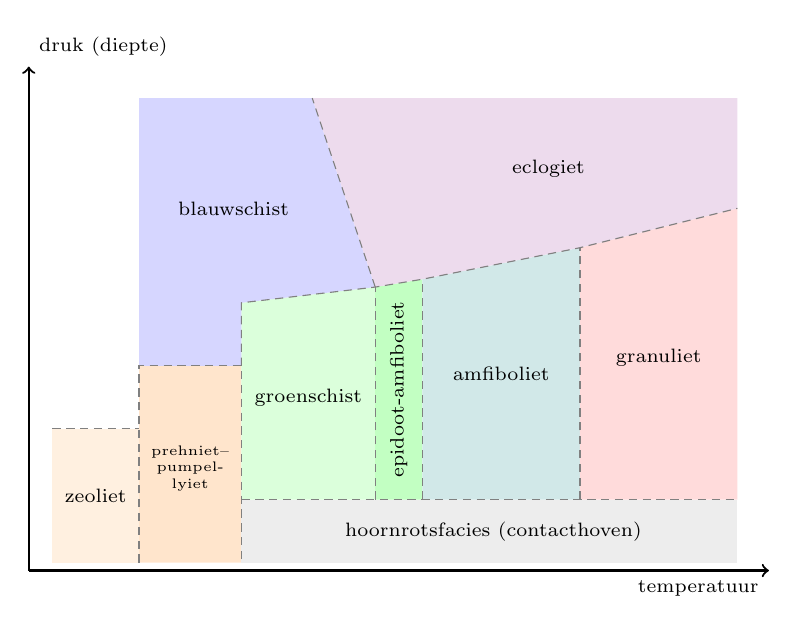
\begin{tikzpicture}[font=\scriptsize, x=1cm, y=1cm]
\draw[->, thick] (0,0) -- (9.4,0) node[below left] {temperatuur};
\draw[->, thick] (0,0) -- (0,6.4) node[above right] {druk (diepte)};
\fill[orange!12] (0.3,0.1) -- (1.4,0.1) -- (1.4,1.8) -- (0.3,1.8) -- cycle;
\fill[orange!20] (1.4,0.1) -- (2.7,0.1) -- (2.7,2.6) -- (1.4,2.6) -- (1.4,1.8) -- cycle;
\fill[green!14] (2.7,0.9) -- (4.4,0.9) -- (4.4,3.6) -- (2.7,3.4) -- cycle;
\fill[green!24] (4.4,0.9) -- (5.0,0.9) -- (5.0,3.7) -- (4.4,3.6) -- cycle;
\fill[teal!18] (5.0,0.9) -- (7.0,0.9) -- (7.0,4.1) -- (5.0,3.7) -- cycle;
\fill[red!14] (7.0,0.9) -- (9.0,0.9) -- (9.0,4.6) -- (7.0,4.1) -- cycle;
\fill[gray!14] (2.7,0.1) -- (9.0,0.1) -- (9.0,0.9) -- (2.7,0.9) -- cycle;
\fill[blue!16] (1.4,2.6) -- (2.7,2.6) -- (2.7,3.4) -- (4.4,3.6) -- (3.6,6.0) -- (1.4,6.0) -- cycle;
\fill[violet!14] (4.4,3.6) -- (5.0,3.7) -- (7.0,4.1) -- (9.0,4.6) -- (9.0,6.0) -- (3.6,6.0) -- cycle;
\draw[gray, densely dashed] (1.4,0.1) -- (1.4,2.6) -- (2.7,2.6) -- (2.7,0.1);
\draw[gray, densely dashed] (0.3,1.8) -- (1.4,1.8);
\draw[gray, densely dashed] (2.7,0.9) -- (9.0,0.9);
\draw[gray, densely dashed] (4.4,0.9) -- (4.4,3.6) (5.0,0.9) -- (5.0,3.7) (7.0,0.9) -- (7.0,4.1);
\draw[gray, densely dashed] (2.7,2.6) -- (2.7,3.4) -- (4.4,3.6) -- (5.0,3.7) -- (7.0,4.1) -- (9.0,4.6);
\draw[gray, densely dashed] (4.4,3.6) -- (3.6,6.0);
\node at (0.85,0.95) {zeoliet};
\node[align=center, font=\tiny] at (2.05,1.3) {prehniet--\\pumpel-\\lyiet};
\node at (3.55,2.2) {groenschist};
\node[rotate=90] at (4.7,2.3) {epidoot-amfiboliet};
\node at (6.0,2.5) {amfiboliet};
\node at (8.0,2.7) {granuliet};
\node at (5.9,0.5) {hoornrotsfacies (contacthoven)};
\node at (2.6,4.6) {blauwschist};
\node at (6.6,5.1) {eclogiet};
\end{tikzpicture}
\par\smallskip{\small Het \omterm{def:b2:metamorphic-facies:facies}{faciesrooster}, schematisch: de volgorde van de facies uit de tabel in
het druk--temperatuurvlak. De grenzen zijn geleidelijk en bewust zonder getallen
getekend: de facies worden gedefinieerd door associaties, en de reacties die ze begrenzen, hangen
af van de samenstelling van elk gesteente.}
\end{omfigure}
% ledger: scmr:facies, scmr:facies-assemblages

\begin{omfigure}
\centering
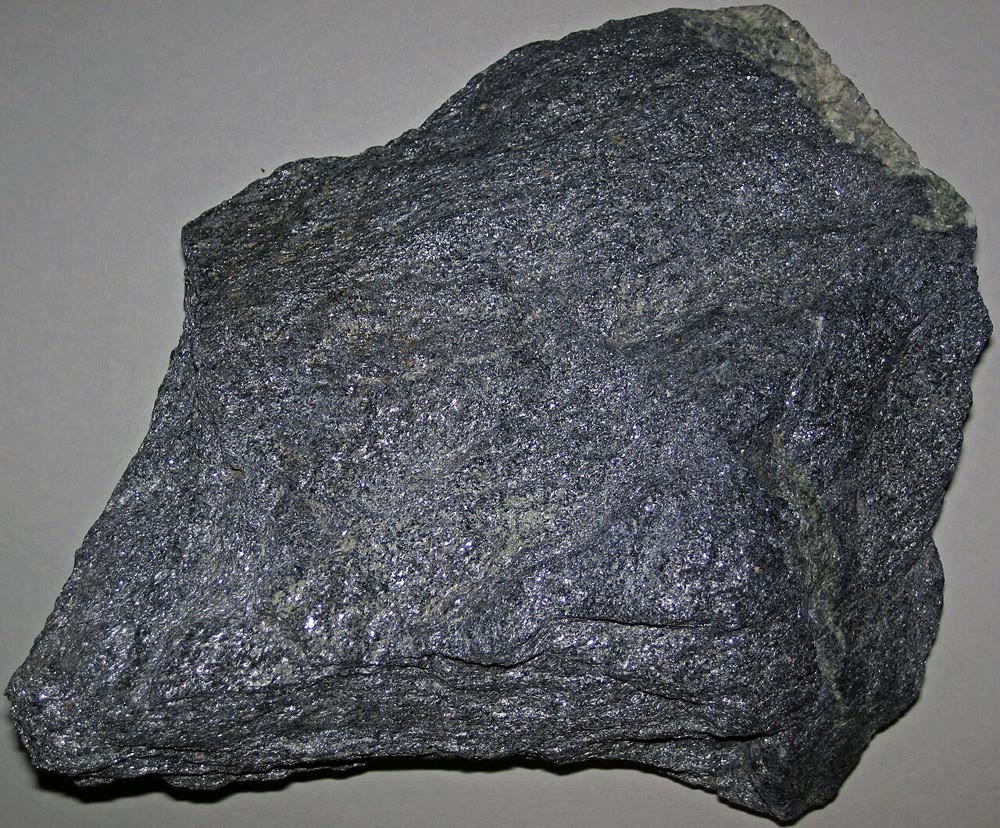
\includegraphics[width=0.27\linewidth]{images/book4/b2-10-blueschist.jpg}\hspace{0.02\linewidth}%
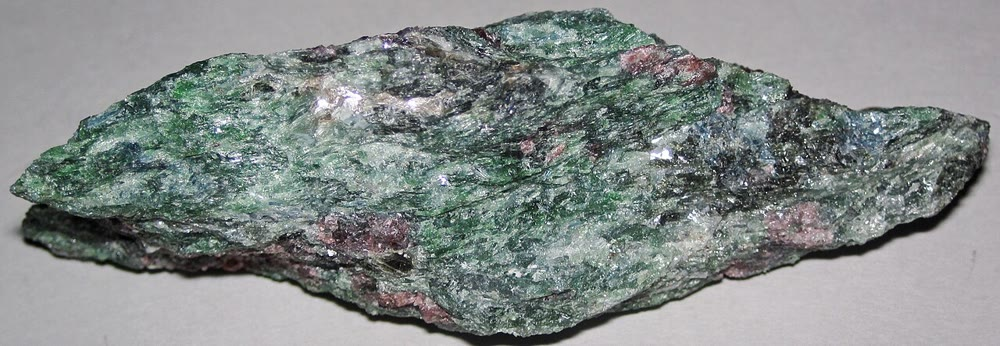
\includegraphics[width=0.69\linewidth]{images/book4/b2-10-eclogite.jpg}
\par\smallskip{\small Twee gemetamorfoseerde basalten. Links: een lawsonietblauwschist uit het
Franciscan Complex in Californië, blauw van glaucofaan. Rechts: een eclogiet uit
West-Noorwegen, groen omfaciet en rode granaat met wat kwarts, kyaniet en rutiel. Foto's
James St.~John, CC BY 2.0.}
\end{omfigure}

Gesteenten die samen worden begraven en verhit, doorlopen de facies in een regelmatige volgorde, die
de verhouding van druk tot temperatuur langs hun pad weerspiegelt: hoog in een
subductiezone, waar blauwschisten ontstaan; gemiddeld in een botsingsgordel; laag bij een intrusie.
\Cref{ch:b2:pt-paths} benoemt deze reeksen en leest zulke paden af uit mineralen.
% ledger: scmr:facies

\section{De protoliet doet ertoe}\label{sec:b2:metamorphic-facies:protoliths}

De facies zijn gedefinieerd aan de hand van basalten, maar elke \omterm{def:b2:metamorphic-facies:metamorphism}{protoliet} legt dezelfde omstandigheden vast in
zijn eigen mineralen.

\begin{definition}[Metapeliet; metabasiet]\label{def:b2:metamorphic-facies:protoliths}
Een \emph{metapeliet}\index{metapeliet} is een gemetamorfoseerde kleisteen (een peliet), rijk aan
aluminium en kalium, waarvan de associaties mica's, chloriet, granaat, stauroliet en
de aluminiumsilicaten bevatten. Een \emph{metabasiet}\index{metabasiet} is een gemetamorfoseerde basalt,
gabbro of ander mafisch gesteente, rijk aan calcium, magnesium en ijzer, waarvan de associaties
de facies definiëren.
\end{definition}

In een \omterm{def:b2:metamorphic-facies:protoliths}{metapeliet} verschijnen de indexmineralen uit Boek~2 na elkaar naarmate
de graad stijgt (chloriet, biotiet, granaat, stauroliet, kyaniet, sillimaniet), maakt de
reactie muscoviet + kwarts uit dit hoofdstuk bij nog hogere temperatuur sillimaniet en
kaliveldspaat, en vertelt het aanwezige aluminiumsilicaat aan welke kant van het
tripelpunt het gesteente passeerde. Een gemetamorfoseerde kalksteen of dolosteen wordt een marmer, van calciet of
dolomiet; onzuivere carbonaten, met silica en klei, worden kalksilicaatgesteenten waarvan
de decarbonatatiereacties koolstofdioxide vrijmaken; een kwartszandsteen wordt een kwartsiet,
dat weinig meer laat zien dan zijn korrelgrootte. Een \omterm{def:b2:metamorphic-facies:protoliths}{metapeliet} uit de chlorietzone en een
metabasalt ernaast, bij dezelfde druk en temperatuur, lijken in niets op elkaar, de
tweede een groensteen van actinoliet, chloriet, epidoot en albiet: één stel omstandigheden,
twee associaties.
% ledger: iugs:barrow, day73:ms-qz, scmr:facies-assemblages

\section{Oefeningen}

\begin{exercise}[$\star$]\label{exo:b2:metamorphic-facies:1}
Benoem het type \omterm{def:b2:metamorphic-facies:metamorphism}{metamorfose}: (a) een kalksteen die binnen \qty{500}{m} van een graniet
tot marmer is geherkristalliseerd; (b) een fijnkorrelig, gebande gesteente langs een grote horizontale
schuifbreuk, met verbrijzelde en geherkristalliseerde korrels; (c) een basalt van de oceaankorst waarvan
het glas bij een rug in chloriet en zeolieten is omgezet, met zijn mineralen slechts gedeeltelijk
vervangen; (d) vulkanische zandstenen onderaan een pakket van \qty{10}{km} dik,
geherkristalliseerd zonder schistositeit.
\end{exercise}
% ledger: scmr:types

\begin{exercise}[$\star$]\label{exo:b2:metamorphic-facies:2}
Bereken uit de tabel van de aluminiumsilicaten $\Delta_r S$, $\Delta_r V$ en de
\omterm{def:b2:metamorphic-facies:clapeyron}{Clapeyronhelling} van kyaniet $\to$ sillimaniet, in \unit{bar/K} en in \unit{MPa/K}. Bepaal hoeveel
de evenwichtsdruk verandert over \qty{100}{\celsius}.
\end{exercise}
% ledger: rh95:al2sio5

\begin{exercise}[$\star$]\label{exo:b2:metamorphic-facies:3}
Bepaal tot welke facies elk metabasalt behoort: (a) actinoliet, albiet, chloriet en
epidoot; (b) glaucofaan en lawsoniet; (c) hoornblende en plagioklaas met
\qty{30}{\percent} anorthiet; (d) omfaciet en granaat, geen plagioklaas.
\end{exercise}
% ledger: scmr:facies-assemblages

\begin{exercise}[$\star$]\label{exo:b2:metamorphic-facies:4}
(a) Bereken uit de molaire massa \qty{162.046}{g.mol^{-1}} en de molaire volumes 44.15, 51.52 en
\qty{49.86}{cm^3.mol^{-1}} de dichtheden van kyaniet, andalusiet en sillimaniet.
(b) Welke bevoordeelt druk, en waarom? (c) Mineraaldatabanken geven 3.61, 3.15 en
\qty{3.24}{g.cm^{-3}}: waarom kunnen natuurlijke kristallen van de zuivere fasen afwijken?
\end{exercise}
% ledger: rh95:al2sio5, webmineral:polymorphs

\begin{exercise}[$\star\star$]\label{exo:b2:metamorphic-facies:5}
Voor kyaniet $\to$ andalusiet geldt $\Delta_r H = \qty{3.9}{kJ}$, $\Delta_r S =
\qty{8.59}{J.K^{-1}}$, $\Delta_r V = \qty{0.737}{J.bar^{-1}}$. (a) Bepaal welke polymorf
stabiel is bij \qty{25}{\celsius} en \qty{1}{bar}. (b) Bepaal bij welke temperatuur de twee
bij \qty{1}{bar} naast elkaar bestaan. (c) Bereken de evenwichtsdruk bij \qty{400}{\celsius} en
vergelijk met de experimentele \qty{2.54}{kbar}. (d) Waarom wordt andalusiet toch
gevonden in gesteenten die tot aan het oppervlak zijn afgekoeld?
\end{exercise}
% ledger: rh95:al2sio5, hm93:table11

\begin{exercise}[$\star\star$]\label{exo:b2:metamorphic-facies:6}
Toets stap (2) van de methode. Bij \qty{1000}{K} geven de tabellen $S_T$ = 285.02 voor kyaniet
en 296.44 voor sillimaniet, en $(H_T - H_{298})/T$ = 122.29 en 121.39
(\unit{J.mol^{-1}.K^{-1}}). (a) Bereken $\Delta_r H$, $\Delta_r S$ en $\Delta_r G$ van
kyaniet $\to$ sillimaniet bij \qty{1000}{K} en \qty{1}{bar}. (b) Vergelijk met de constante
waarden van de tabel. (c) Bepaal welke polymorf daar stabiel is, en hoe groot de fout van
de eenvoudige methode is.
\end{exercise}
% ledger: rh95:al2sio5-ht, rh95:al2sio5

\begin{exercise}[$\star\star$]\label{exo:b2:metamorphic-facies:7}
Calciet en aragoniet (\ce{CaCO3}) hebben bij \qty{298.15}{K} $\Delta_f G$ = $-1128.5$ en
$-1127.4$ \unit{kJ.mol^{-1}}, $S$ = 91.7 en 88.0 \unit{J.mol^{-1}.K^{-1}}, $V$ = 36.93
en \qty{34.15}{cm^3.mol^{-1}}, en gelijke vormingsenthalpieën. (a) Bepaal de
evenwichtsdruk bij \qty{25}{\celsius}. (b) Bereken de \omterm{def:b2:metamorphic-facies:clapeyron}{Clapeyronhelling}. (c) Bepaal de
evenwichtsdruk bij \qty{300}{\celsius}. (d) Veel schelpen bestaan uit aragoniet en
leven bij \qty{1}{bar}: wat zegt dat?
\end{exercise}
% ledger: rh95:cc-ar

\begin{exercise}[$\star\star$]\label{exo:b2:metamorphic-facies:8}
Voor albiet $\to$ jadeïet + kwarts geven de tabellen $\Delta_r H = \qty{-5.0}{kJ}$,
$\Delta_r S = \qty{-32.4}{J.K^{-1}}$, $\Delta_r V = \qty{-1.698}{J.bar^{-1}}$. (a)
Bereken de \omterm{def:b2:metamorphic-facies:clapeyron}{Clapeyronhelling}. (b) Bereken de evenwichtsdruk bij \qty{500}{\celsius}.
(c) De vormingsenthalpieën van albiet, jadeïet en kwarts zijn onzeker tot op 2.6, 3.6
en \qty{1.0}{kJ.mol^{-1}}; bepaal, door ze als onafhankelijke fouten te combineren, hoe onzeker die
druk is. (d) Waarom ontbreekt plagioklaas in de eclogietfacies?
\end{exercise}
% ledger: rh95:ab-jd-qz, scmr:facies-assemblages

\begin{exercise}[$\star\star$]\label{exo:b2:metamorphic-facies:9}
Muscoviet + kwarts valt uiteen bij 603, 637 en \qty{662}{\celsius} bij 1, 2 en
\qty{3}{kbar}. (a) Bereken de helling van de lijn tussen elk paar punten. (b) Bepaal, als de
reactie-entropie over dit bereik nauwelijks verandert, met welke factor $\Delta_r V$
kromp van het eerste interval naar het tweede. (c) Welke fase is verantwoordelijk?
\end{exercise}
% ledger: day73:ms-qz

\begin{exercise}[$\star\star\star$]\label{exo:b2:metamorphic-facies:10}
Met de constante eigenschappen van de methode: (a) bereken de drukken van de drie
reacties bij \qty{600}{\celsius}; (b) toon aan dat bij \qty{600}{\celsius} en de druk van
kyaniet $=$ andalusiet sillimaniet de stabielste polymorf is, zodat dit punt van
de lijn metastabiel is; (c) bepaal welke polymorf stabiel is bij \qty{600}{\celsius} en
\qty{4}{kbar}, en bij \qty{600}{\celsius} en \qty{7}{kbar}.
\end{exercise}
% ledger: rh95:al2sio5

\begin{exercise}[$\star\star\star$]\label{exo:b2:metamorphic-facies:11}
Een schist bevat kyaniet, andalusiet en sillimaniet samen, alle drie in
evenwicht gegroeid. (a) Bepaal met het experimentele tripelpunt, $504 \pm \qty{20}{\celsius}$ en
$3.75 \pm \qty{0.25}{kbar}$, en een korst met dichtheid \qty{2700}{kg.m^{-3}} ($g =
\qty{9.81}{m.s^{-2}}$), op welke diepte hij groeide. (b) Bepaal, met \qty{10}{\celsius} aan het
oppervlak, welke gemiddelde thermische gradiënt dat inhoudt. (c) Waarom zijn zulke gesteenten zeldzaam?
\end{exercise}
% ledger: hm93:triple

\begin{exercise}[$\star\star\star$]\label{exo:b2:metamorphic-facies:12}
Twee gesteenten worden tot diepte $z$ begraven, vanaf \qty{10}{\celsius} aan het oppervlak: gesteente X langs
\qty{10}{\celsius.km^{-1}} tot \qty{30}{km} onder gesteenten met gemiddelde dichtheid
\qty{3000}{kg.m^{-3}}, gesteente Y langs \qty{30}{\celsius.km^{-1}} tot \qty{20}{km} onder gesteenten
met gemiddelde dichtheid \qty{2800}{kg.m^{-3}}. (a) Bereken $T$ en $P$ aan het eind van elk pad.
(b) Bepaal met de lijnen voor constante eigenschappen (calciet $=$ aragoniet: $P = 13.31\,T$ bar met $T$
in kelvin; albiet $=$ jadeïet + kwarts uit \cref{exo:b2:metamorphic-facies:8}; de aluminiumsilicaten uit de
tabel) of elk gesteente aragoniet of calciet bevat, jadeïet + kwarts of albiet, en welk
aluminiumsilicaat. (c) Welk pad is het koudere hogedrukpad, en in welke facies eindigt elk?
\end{exercise}
% ledger: rh95:cc-ar, rh95:ab-jd-qz, rh95:al2sio5

\section{Probleem: Het tripelpunt opbouwen}

\begin{problem}[{Weekendprobleem --- het aluminiumsilicaatdiagram uit de tabellen, en hoever
het te vertrouwen is}]
\label{pb:b2:metamorphic-facies:1}
Gebruik de tabel van de aluminiumsilicaten (\qty{298.15}{K}, \qty{1}{bar}) en de methode van
dit hoofdstuk, met constante $\Delta_r H$, $\Delta_r S$ en $\Delta_r V$; schrijf $T$ in
kelvin, $P$ in bar, en verwaarloos de 1 in $P - 1$.

\noindent\textbf{Deel I --- De reacties.}
\begin{enumerate}
\item Bereken $\Delta_r H$, $\Delta_r S$ en $\Delta_r V$ voor kyaniet $\to$ andalusiet.
\item Doe hetzelfde voor kyaniet $\to$ sillimaniet.
\item Doe hetzelfde voor andalusiet $\to$ sillimaniet, en ga na dat elke eigenschap het
verschil van de eerste twee is.
\item Zeg welke polymorf de grootste entropie heeft, welke het kleinste volume. Aan welke kant
van elke lijn ligt elk?
\item Bereken de drie \omterm{def:b2:metamorphic-facies:clapeyron}{Clapeyronhellingen}.
\item Waarom is de helling van andalusiet $\to$ sillimaniet negatief?
\end{enumerate}

\noindent\textbf{Deel II --- Waar de lijnen lopen.}
\begin{enumerate}[resume]
\item Bereken $\Delta_r G$ van de eerste twee reacties bij \qty{298.15}{K}. Welke
polymorf is aan het oppervlak stabiel?
\item Bepaal bij welke temperatuur (in \unit{\celsius}) elke reactie bij \qty{1}{bar} het evenwicht
bereikt.
\item Zeg welke van de drie temperaturen van vraag~8 stabiele evenwichten zijn en welke
metastabiele. (Gebruik de volgorde van de drie bij \qty{1}{bar}.)
\item Bereken de druk van kyaniet $=$ andalusiet bij \qty{400}{\celsius}; de
experimenten geven \qty{2.54}{kbar}.
\item Bereken de druk van kyaniet $=$ sillimaniet bij \qty{700}{\celsius}; de
experimenten geven \qty{7.86}{kbar}.
\item Schets de drie lijnen tussen 200 en \qty{900}{\celsius}.
\end{enumerate}

\noindent\textbf{Deel III --- Het tripelpunt.}
\begin{enumerate}[resume]
\item Schrijf de eerste twee lijnen als $P = a_i T - b_i$; geef $a_1$, $b_1$, $a_2$, $b_2$.
\item Bepaal de temperatuur van hun snijpunt.
\item Bereken de druk ervan.
\item Ga na dat andalusiet $=$ sillimaniet erdoorheen gaat.
\item Vergelijk met de experimentele $504 \pm \qty{20}{\celsius}$ en $3.75 \pm
\qty{0.25}{kbar}$.
\item Met de temperatuurafhankelijkheid uit de tabellen verschuift het tripelpunt naar
\qty{536}{\celsius} en \qty{4.20}{kbar}. Bracht de verfijning het dichter bij het
experiment? Wat suggereert dat over de belangrijkste bron van fouten?
\end{enumerate}

\noindent\textbf{Deel IV --- Hoever het te vertrouwen is.}
\begin{enumerate}[resume]
\item Verhoog de vormingsenthalpie van andalusiet met \qty{1}{kJ}. Bepaal hoeveel
de lijn kyaniet $=$ andalusiet bij vaste temperatuur in druk verschuift.
\item Bepaal hoeveel het tripelpunt in temperatuur verschuift.
\item Doe hetzelfde voor een verhoging met \qty{1}{kJ} van de enthalpie van sillimaniet.
\item Elke enthalpie is onzeker tot op \qty{2.0}{kJ}. Bepaal welk bereik van temperaturen van het
tripelpunt de calorimetrische gegevens alleen toelaten.
\item Hoe kunnen thermodynamische tabellen het experimentele diagram dan binnen
\qty{30}{\celsius} reproduceren?
\item Geef de temperatuur van het tripelpunt berekend in Deel III, afgerond op de
graad: het kerngetal van dit probleem.
\end{enumerate}
\end{problem}
% ledger: rh95:al2sio5, rh95:al2sio5-ht, hm93:triple, hm93:table11, hm93:adjusted
